\documentclass[11pt]{article}
\usepackage[margin=1in]{geometry}
\usepackage{amsmath}
\usepackage{graphicx}
\usepackage{booktabs}
\graphicspath{{../Figures/}{../Analysis/}}
\title{Step 4 Result 2.0: Independent Temperature and Field Trends}
\author{}
\date{}
\begin{document}
\maketitle
\section{Purpose of the test}
This report applies the Step 4 validation protocol to the Result 2.0 workflow. The test separates a dimerisation/lattice channel, which follows $\delta(T,B)$, from a scalar spin-correlation proxy $C_1(T,B)$ that remains finite above the spin-Peierls transition.
\section{Physical model}
The active mixing term is
\begin{equation}
H_{\mathrm{mix}} = V_{BD}^{\mathrm{static}} L_{BD} + g_Q^{\mathrm{eff}} Q L_{BD},
\end{equation}
with
\begin{equation}
V_{BD}^{\mathrm{static}} = V_0 + \lambda_\delta \delta(T,B) + \lambda_C C_1(T,B),
\qquad
g_Q^{\mathrm{eff}} = g_{Q0} \delta(T,B) / \delta_{\mathrm{ref}}.
\end{equation}
The dynamic phonon channel therefore turns off when the dimerisation vanishes.
\section{Trend definitions}
The four scenarios are the low-temperature lattice reference, the high-temperature lattice-off control with finite $C_1$, the field-suppressed low-temperature control, and the high-temperature $C_1$-static control. The frequency convention is rephasing $\omega_1 < 0$, unrephasing $\omega_1 > 0$, and $\omega_3 > 0$ for both components. The current grid is $N_w=300$ with rephasing $\omega_1=[-1.1,-0.8]$, unrephasing $\omega_1=[0.8,1.1]$, and $\omega_3=[0.8,1.1]$ eV.
\section{Scenarios and acceptance criteria}
\begin{center}
\begin{tabular}{lrrrrr}
\toprule
Scenario & $\delta$ & $C_1$ & $g_Q^{\mathrm{eff}}$ & $V_{BD}^{\mathrm{static}}$ & $A_{\mathrm{reph}}$ \\
\midrule
lowT\_lattice\_dynamic & 0.00707107 & -0.378667 & 0.01 & 0.02 & 231.909 \\
highT\_lattice\_off\_C1\_finite & 0 & -0.329471 & 0 & 0.01 & 250.111 \\
highB\_lattice\_suppressed & 0 & -0.346199 & 0 & 0.01 & 250.111 \\
highT\_C1\_static & 0 & -0.329471 & 0 & 0.02 & 240.227 \\
\bottomrule
\end{tabular}
\end{center}
The acceptance criteria are that the low-temperature lattice reference has finite $\delta$ and $g_Q^{\mathrm{eff}}$, both high-temperature and high-field lattice-off controls have $\delta=0$ and $g_Q^{\mathrm{eff}}=0$ while retaining finite $C_1$, and the $C_1$-static control demonstrates that a finite scalar channel can persist without dimerisation.
\section{Numerical results}
\begin{figure}[h]
\centering
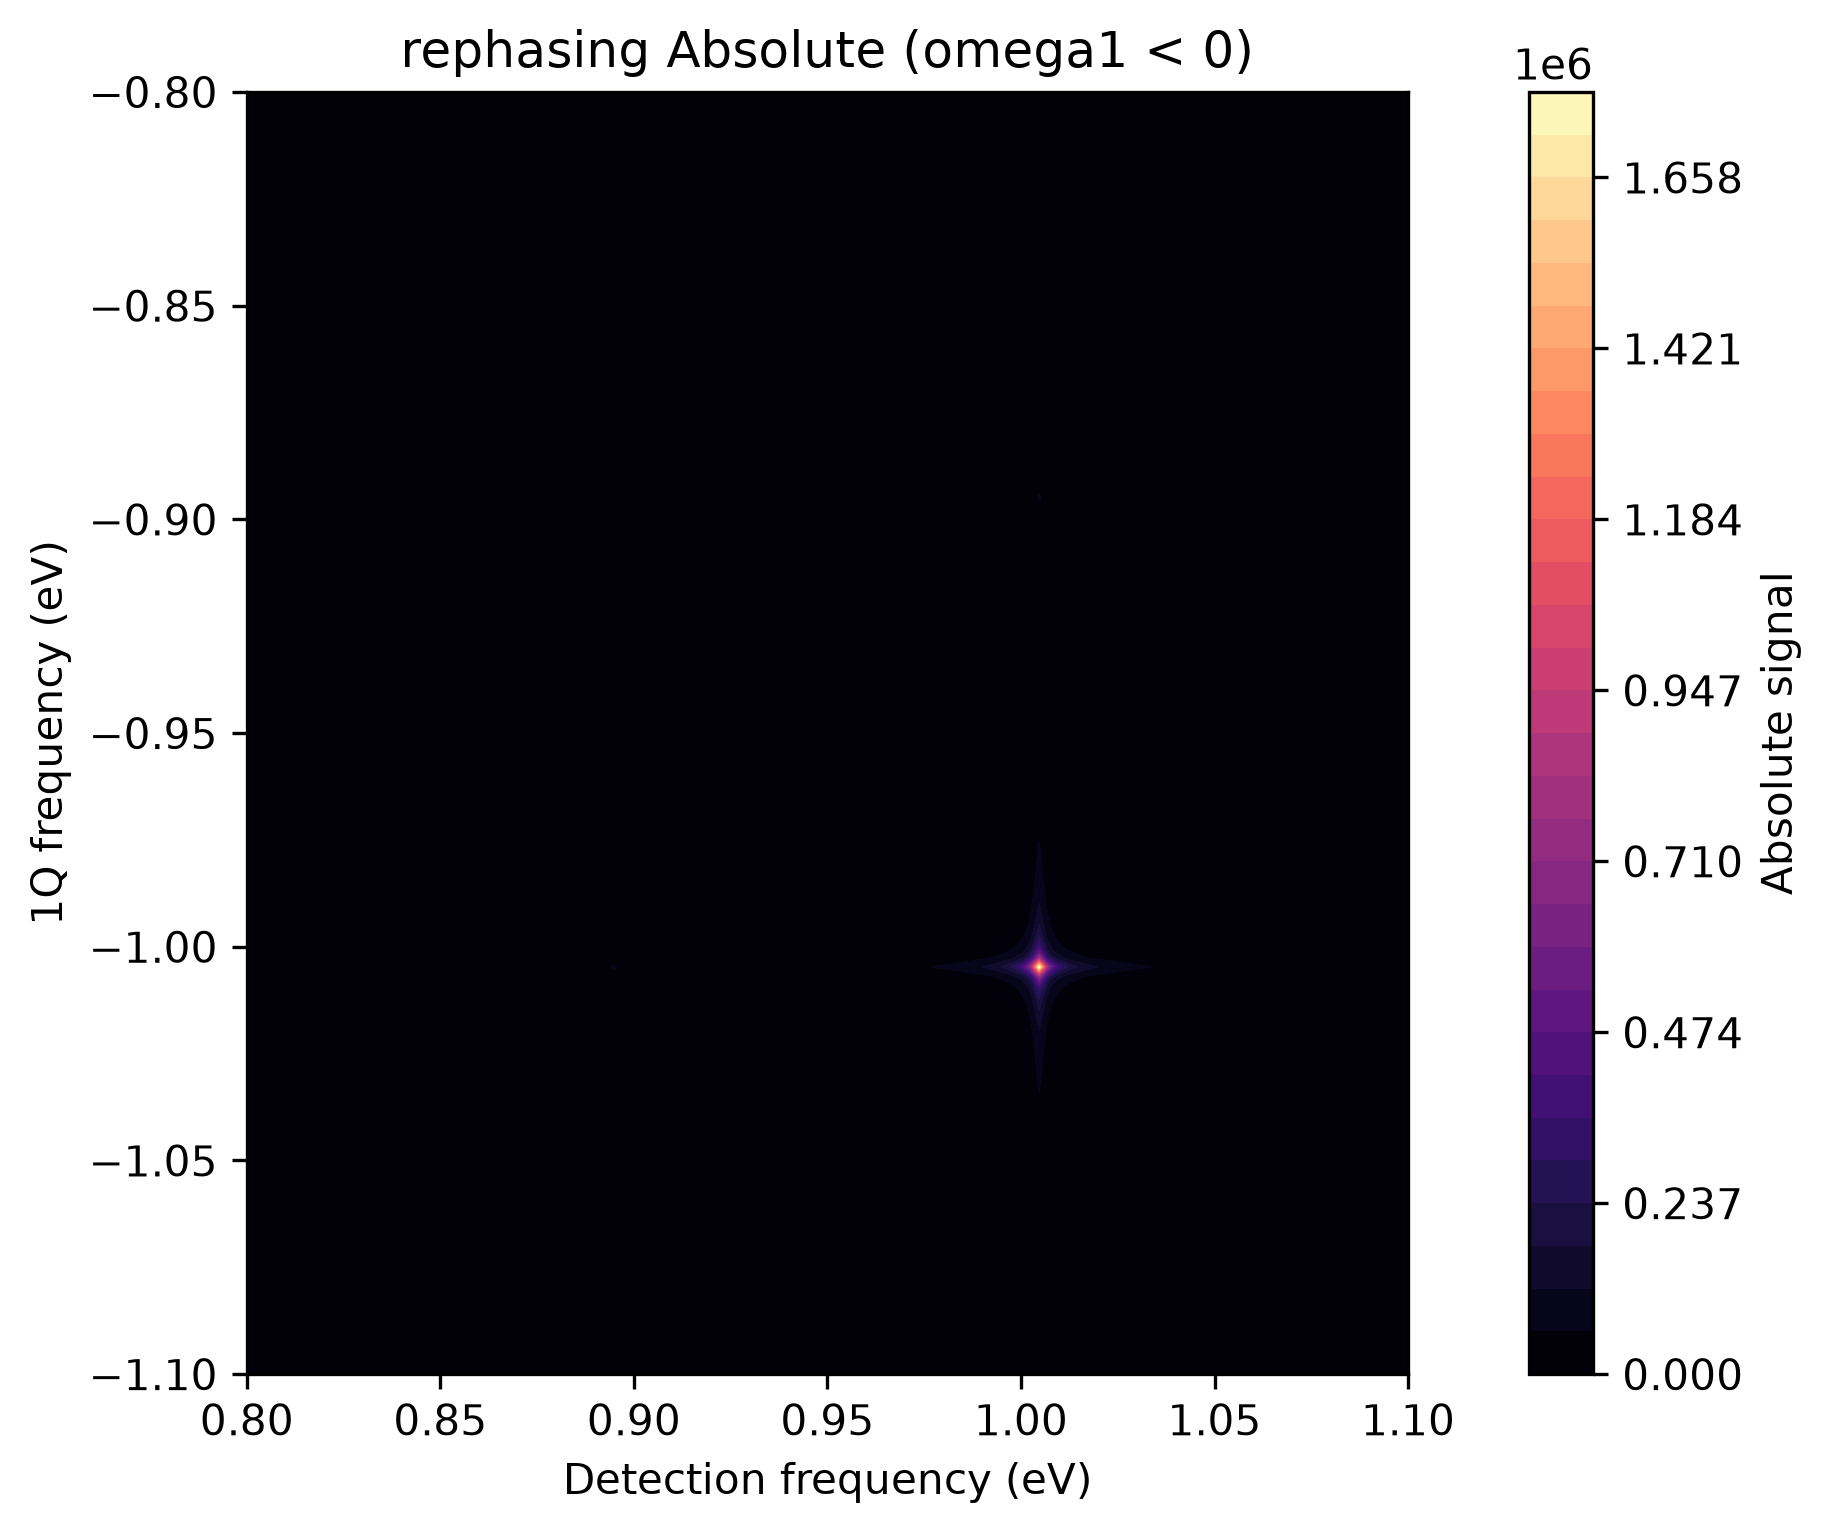
\includegraphics[width=0.48\textwidth]{step04__scenario-000__lowT_lattice_dynamic__T-7K_B-0p0T_rephasing_abs.png}
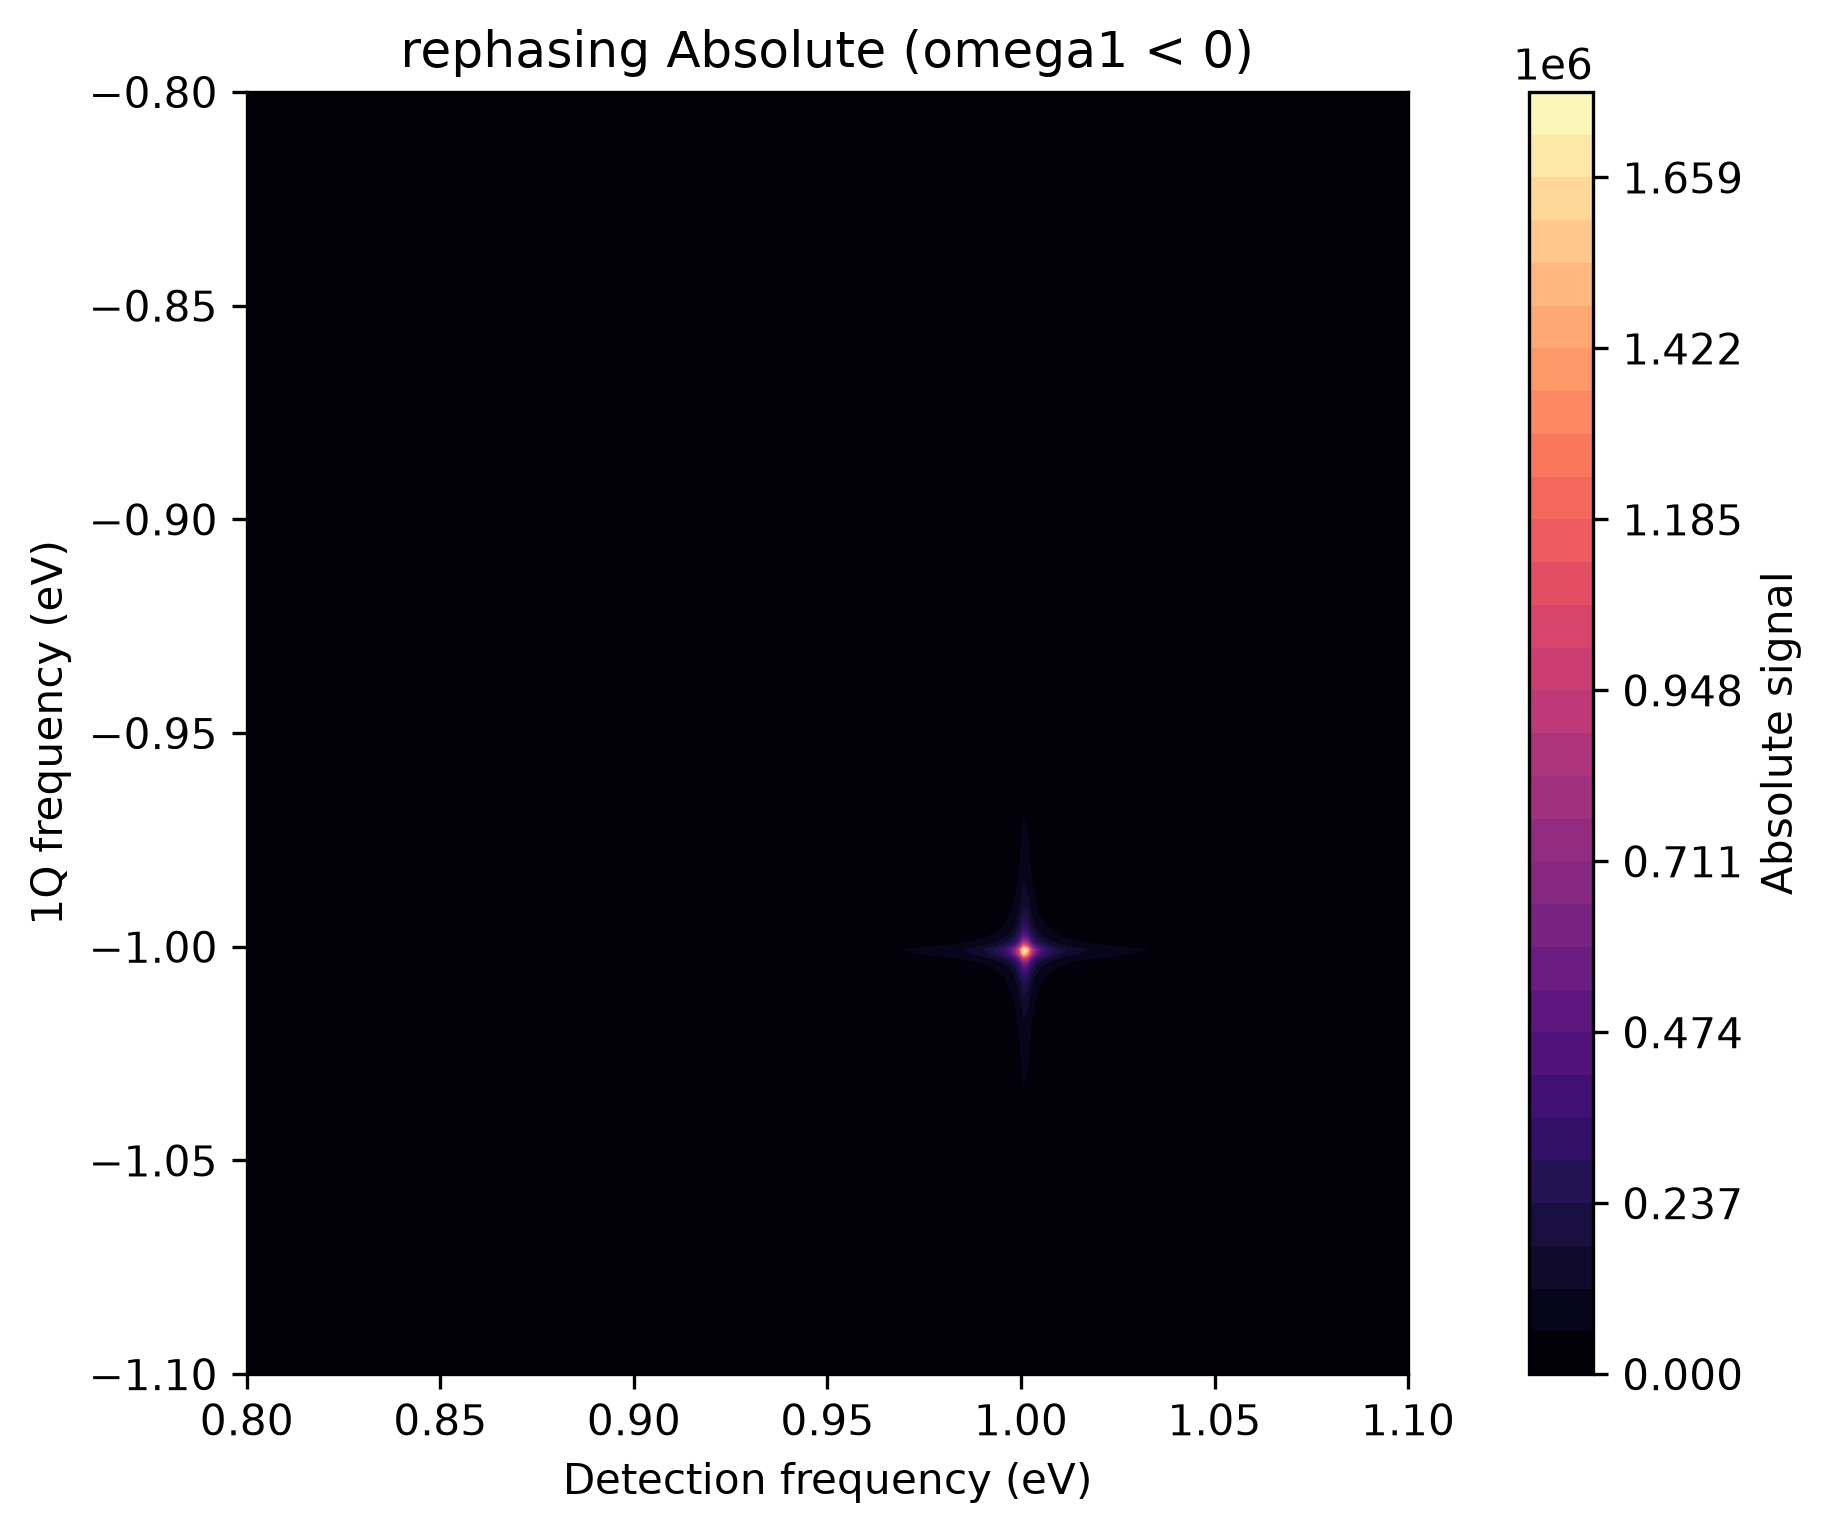
\includegraphics[width=0.48\textwidth]{step04__scenario-001__highT_lattice_off_C1_finite__T-20K_B-0p0T_rephasing_abs.png}
\caption{Representative rephasing absolute spectra. Left: low-temperature lattice dynamic reference. Right: high-temperature lattice-off control.}
\end{figure}
\begin{figure}[h]
\centering
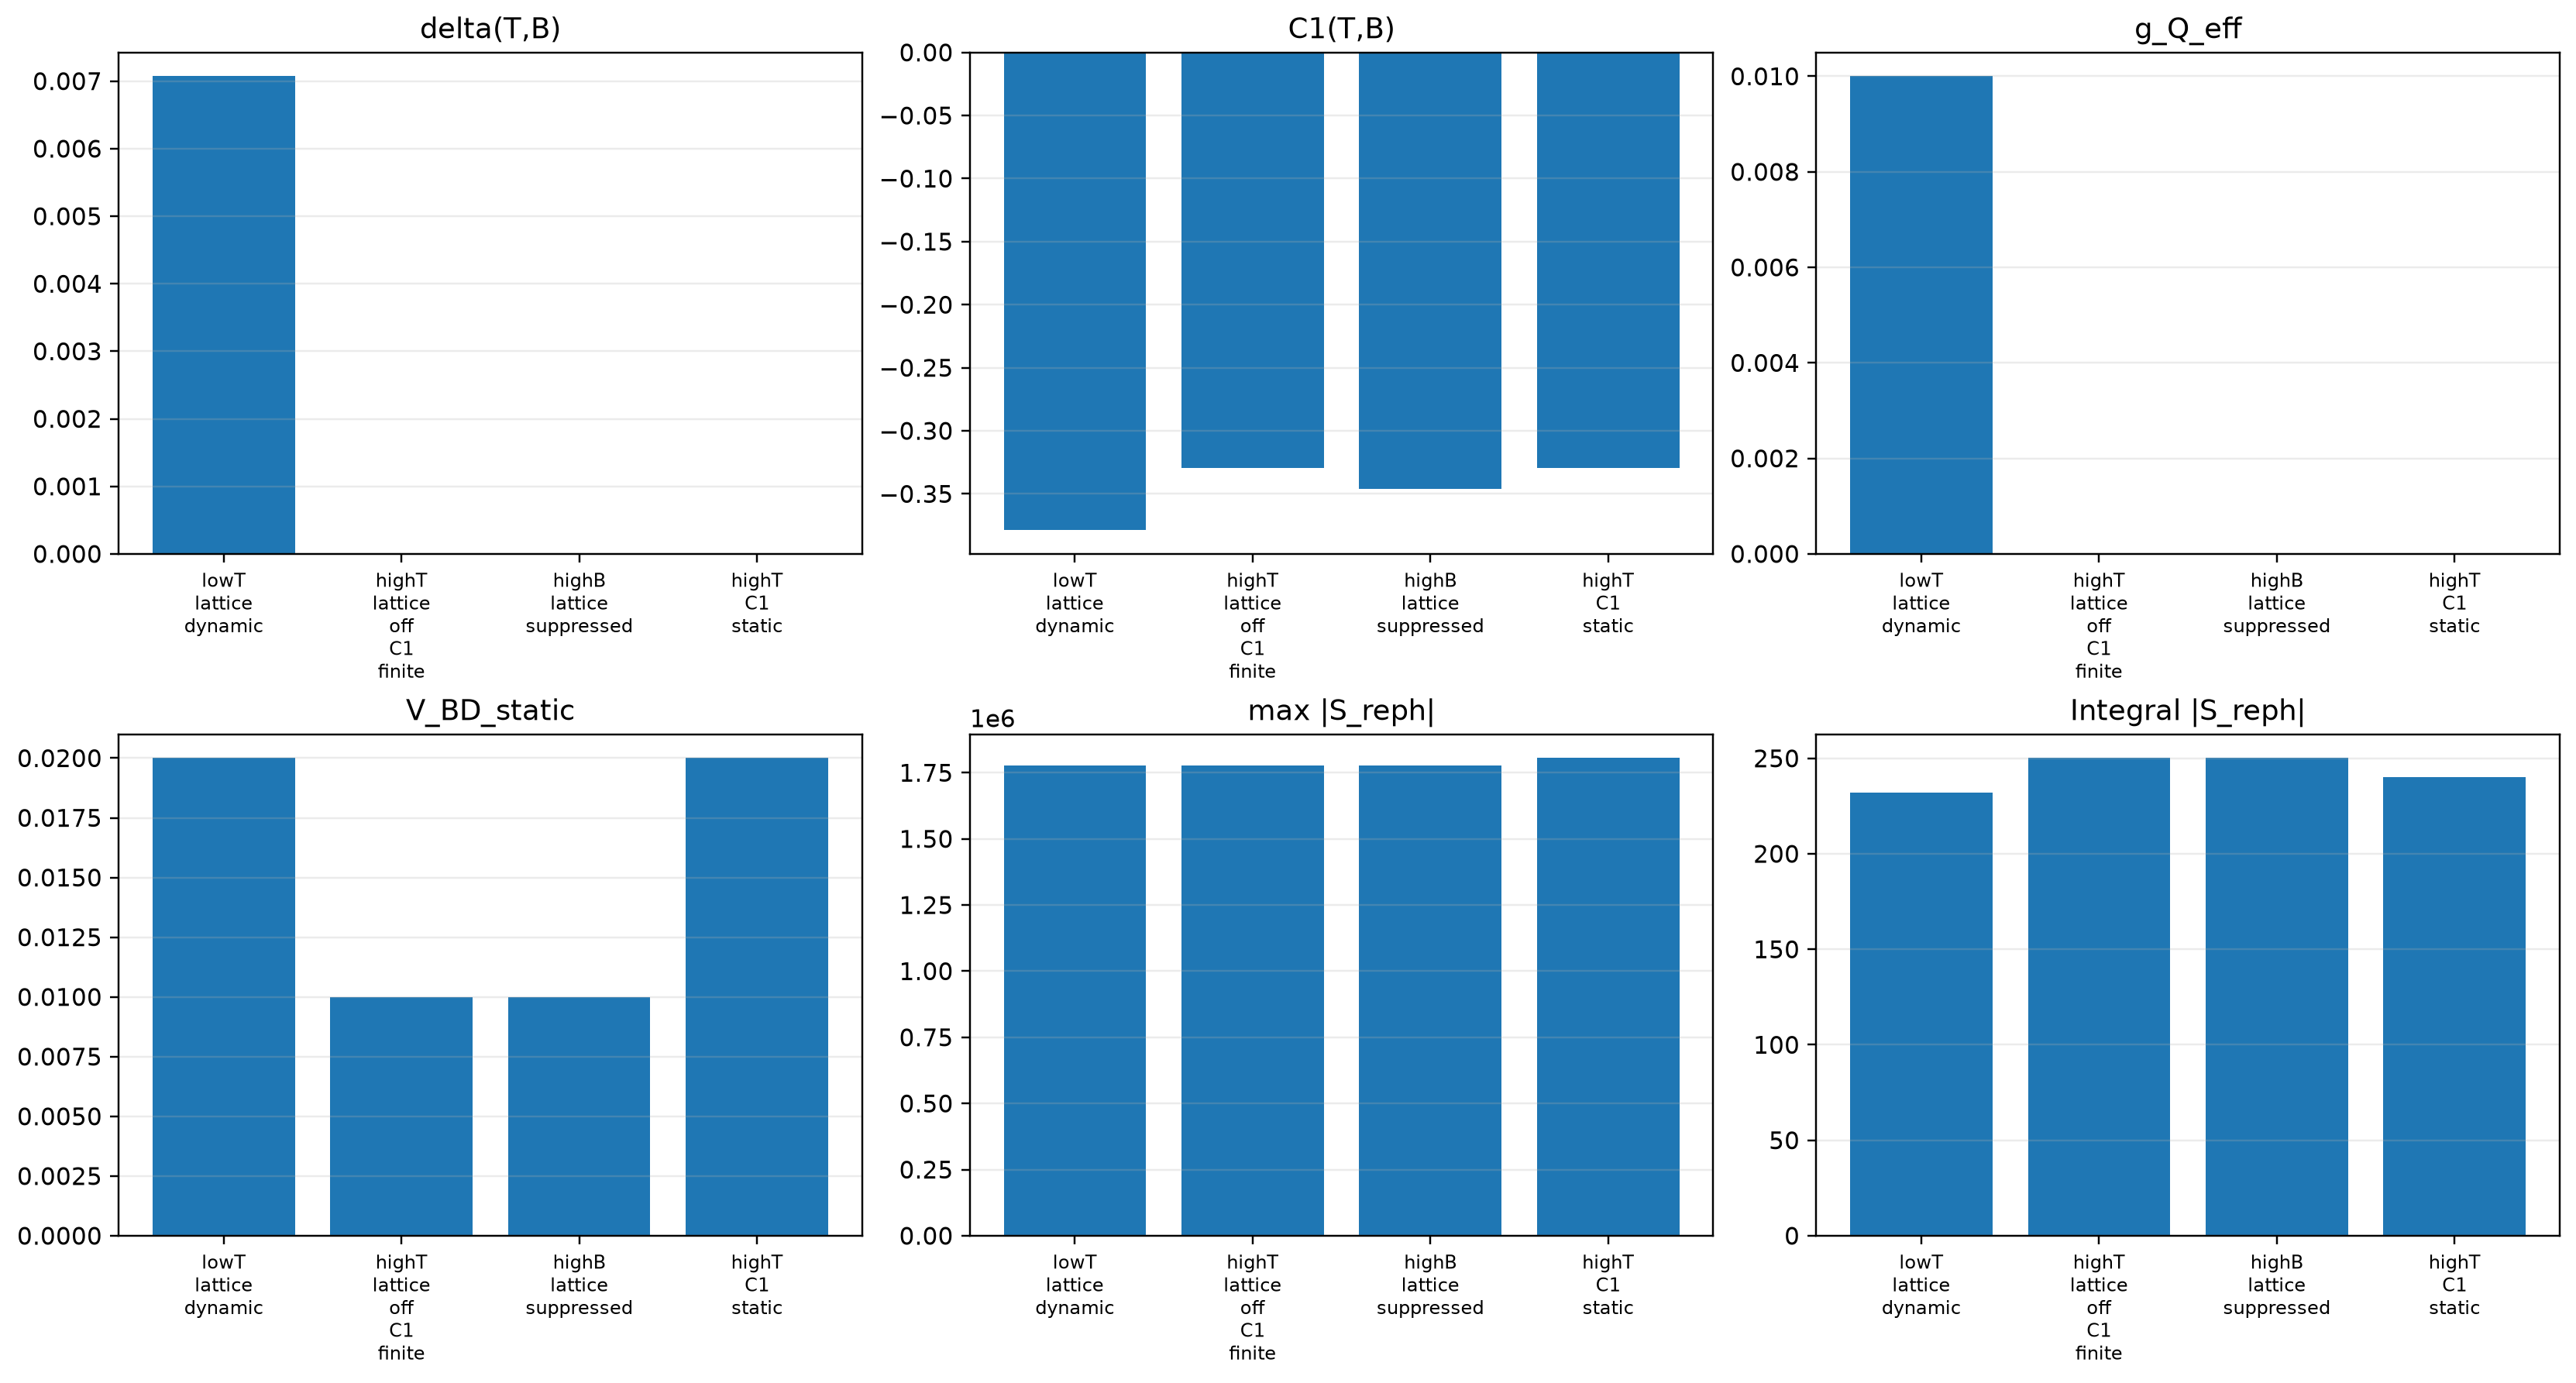
\includegraphics[width=0.82\textwidth]{step04__trend_metrics.png}
\caption{Step 4 trend metrics from the Result 2.0 output files.}
\end{figure}
The analysis files are \verb|step04__scenario_metrics.csv|, \verb|step04__pairwise_differences.csv|, and \verb|step04__validation_outcome.txt| in the \verb|Analysis/| folder.
\section{Validation outcome}
The Step 4 production and trend-control checks pass for the generated scenarios. The high-temperature and high-field controls remove the dynamic lattice channel, while the $C_1$-static case confirms that a persistent scalar contribution should not be interpreted uniquely as evidence of the dimerised phase.
\end{document}
